\section{Präsentationsschicht}\label{sec:praesentationsschicht}

\subsection{Konsolenoberfläche}

Das Modul \texttt{configuration.rest} stellt eine einfache Konsolenoberfläche bereit.
Diese gilt allerdings als veraltet und wird daher im Folgenden nicht näher behandelt.

\subsection{Weboberfläche}

Für die Nutzung von \textit{Vocabduel} existiert eine voll funktionsfähige Webanwendung.
Diese wurde mit \textit{Angular 12} implementiert und folgt modernen Standards.

\subsubsection{Aufbau der Anwendung}

Im Folgenden werden die grundlegenden Features des \textit{Vocabduel}-Frontends erläutert.
Dabei ist jedoch zu erwähnen, dass die Anwendung nicht im Detail beschrieben wird, sondern
an dieser Stelle vielmehr ihr Aufbau und ihr Funktionsumfang skizziert werden.

\begin{figure}[H]
    \centering
    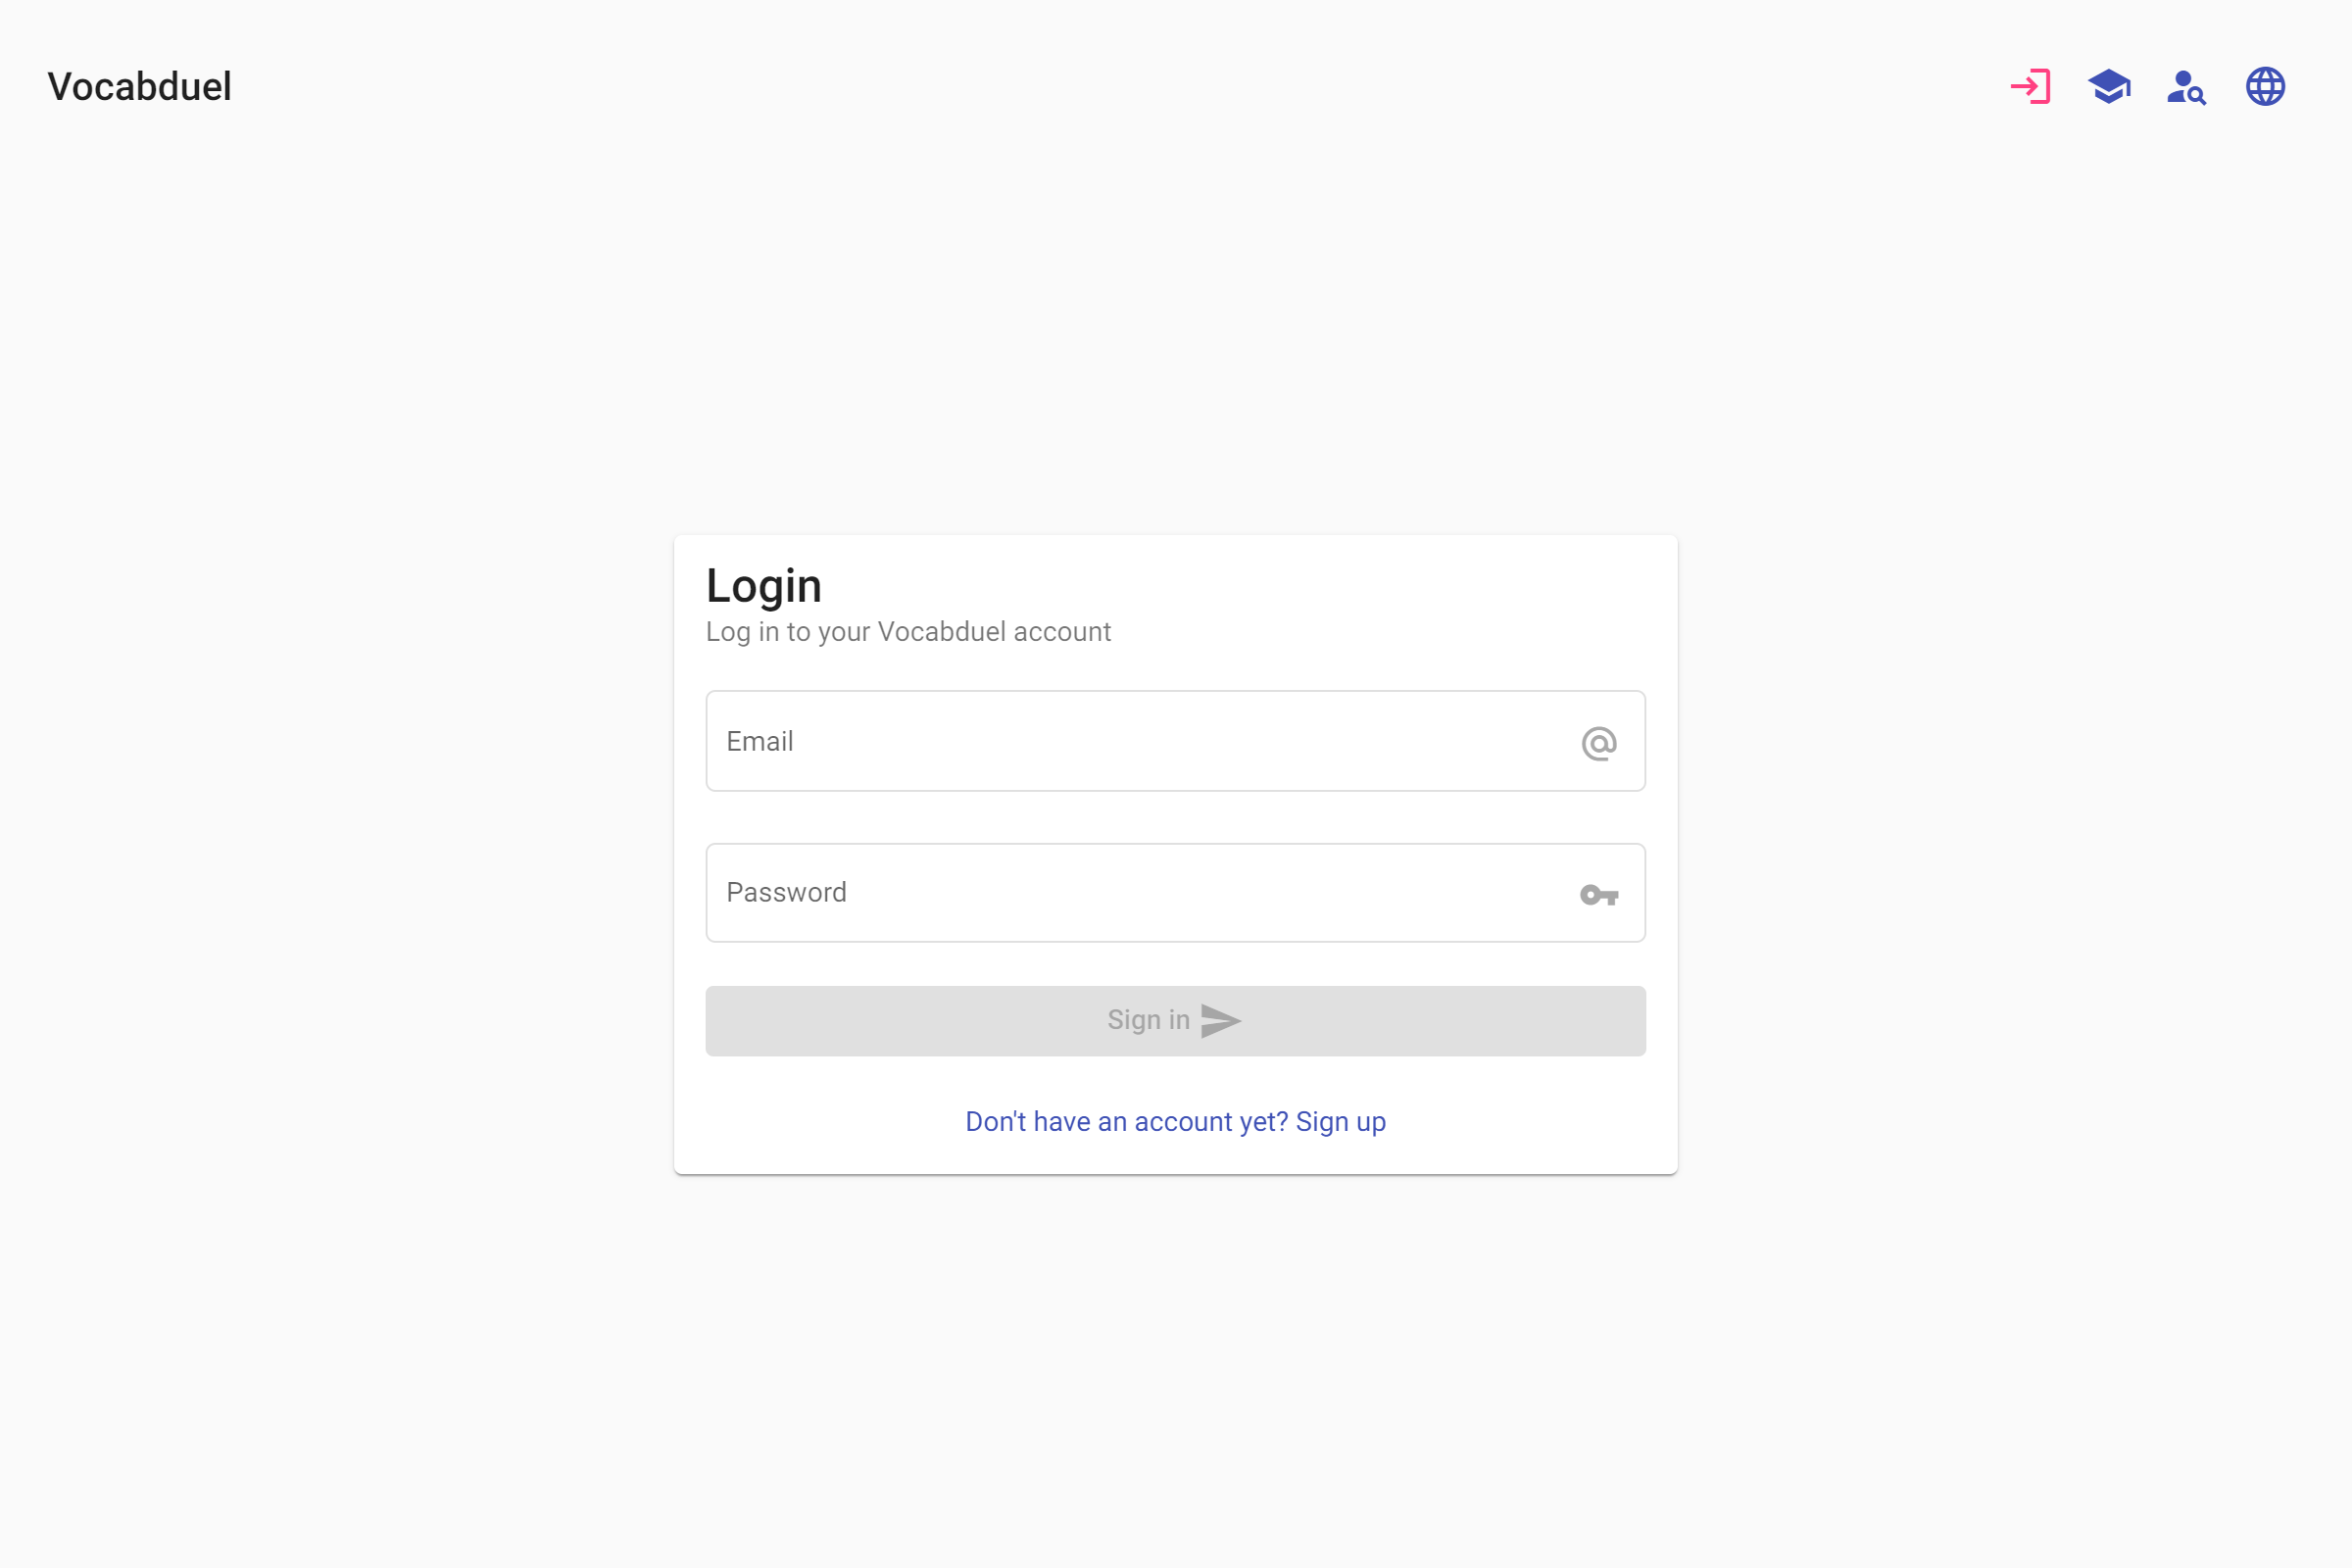
\includegraphics[width=0.8\textwidth]{localhost_8080_app_login}
    \caption[]{Login}
    \label{fig:felogin}
\end{figure}

Die Webanwendung verfügt über eine Oberfläche mithilfe derer man sich im System anmelden kann.
Analog zum Login existiert auch eine Seite zum Erstellen eines Kontos.
Über die Icons in der rechten, oberen Ecke kann zu weiteren Seiten navigiert werden.

\begin{figure}[H]
    \centering
    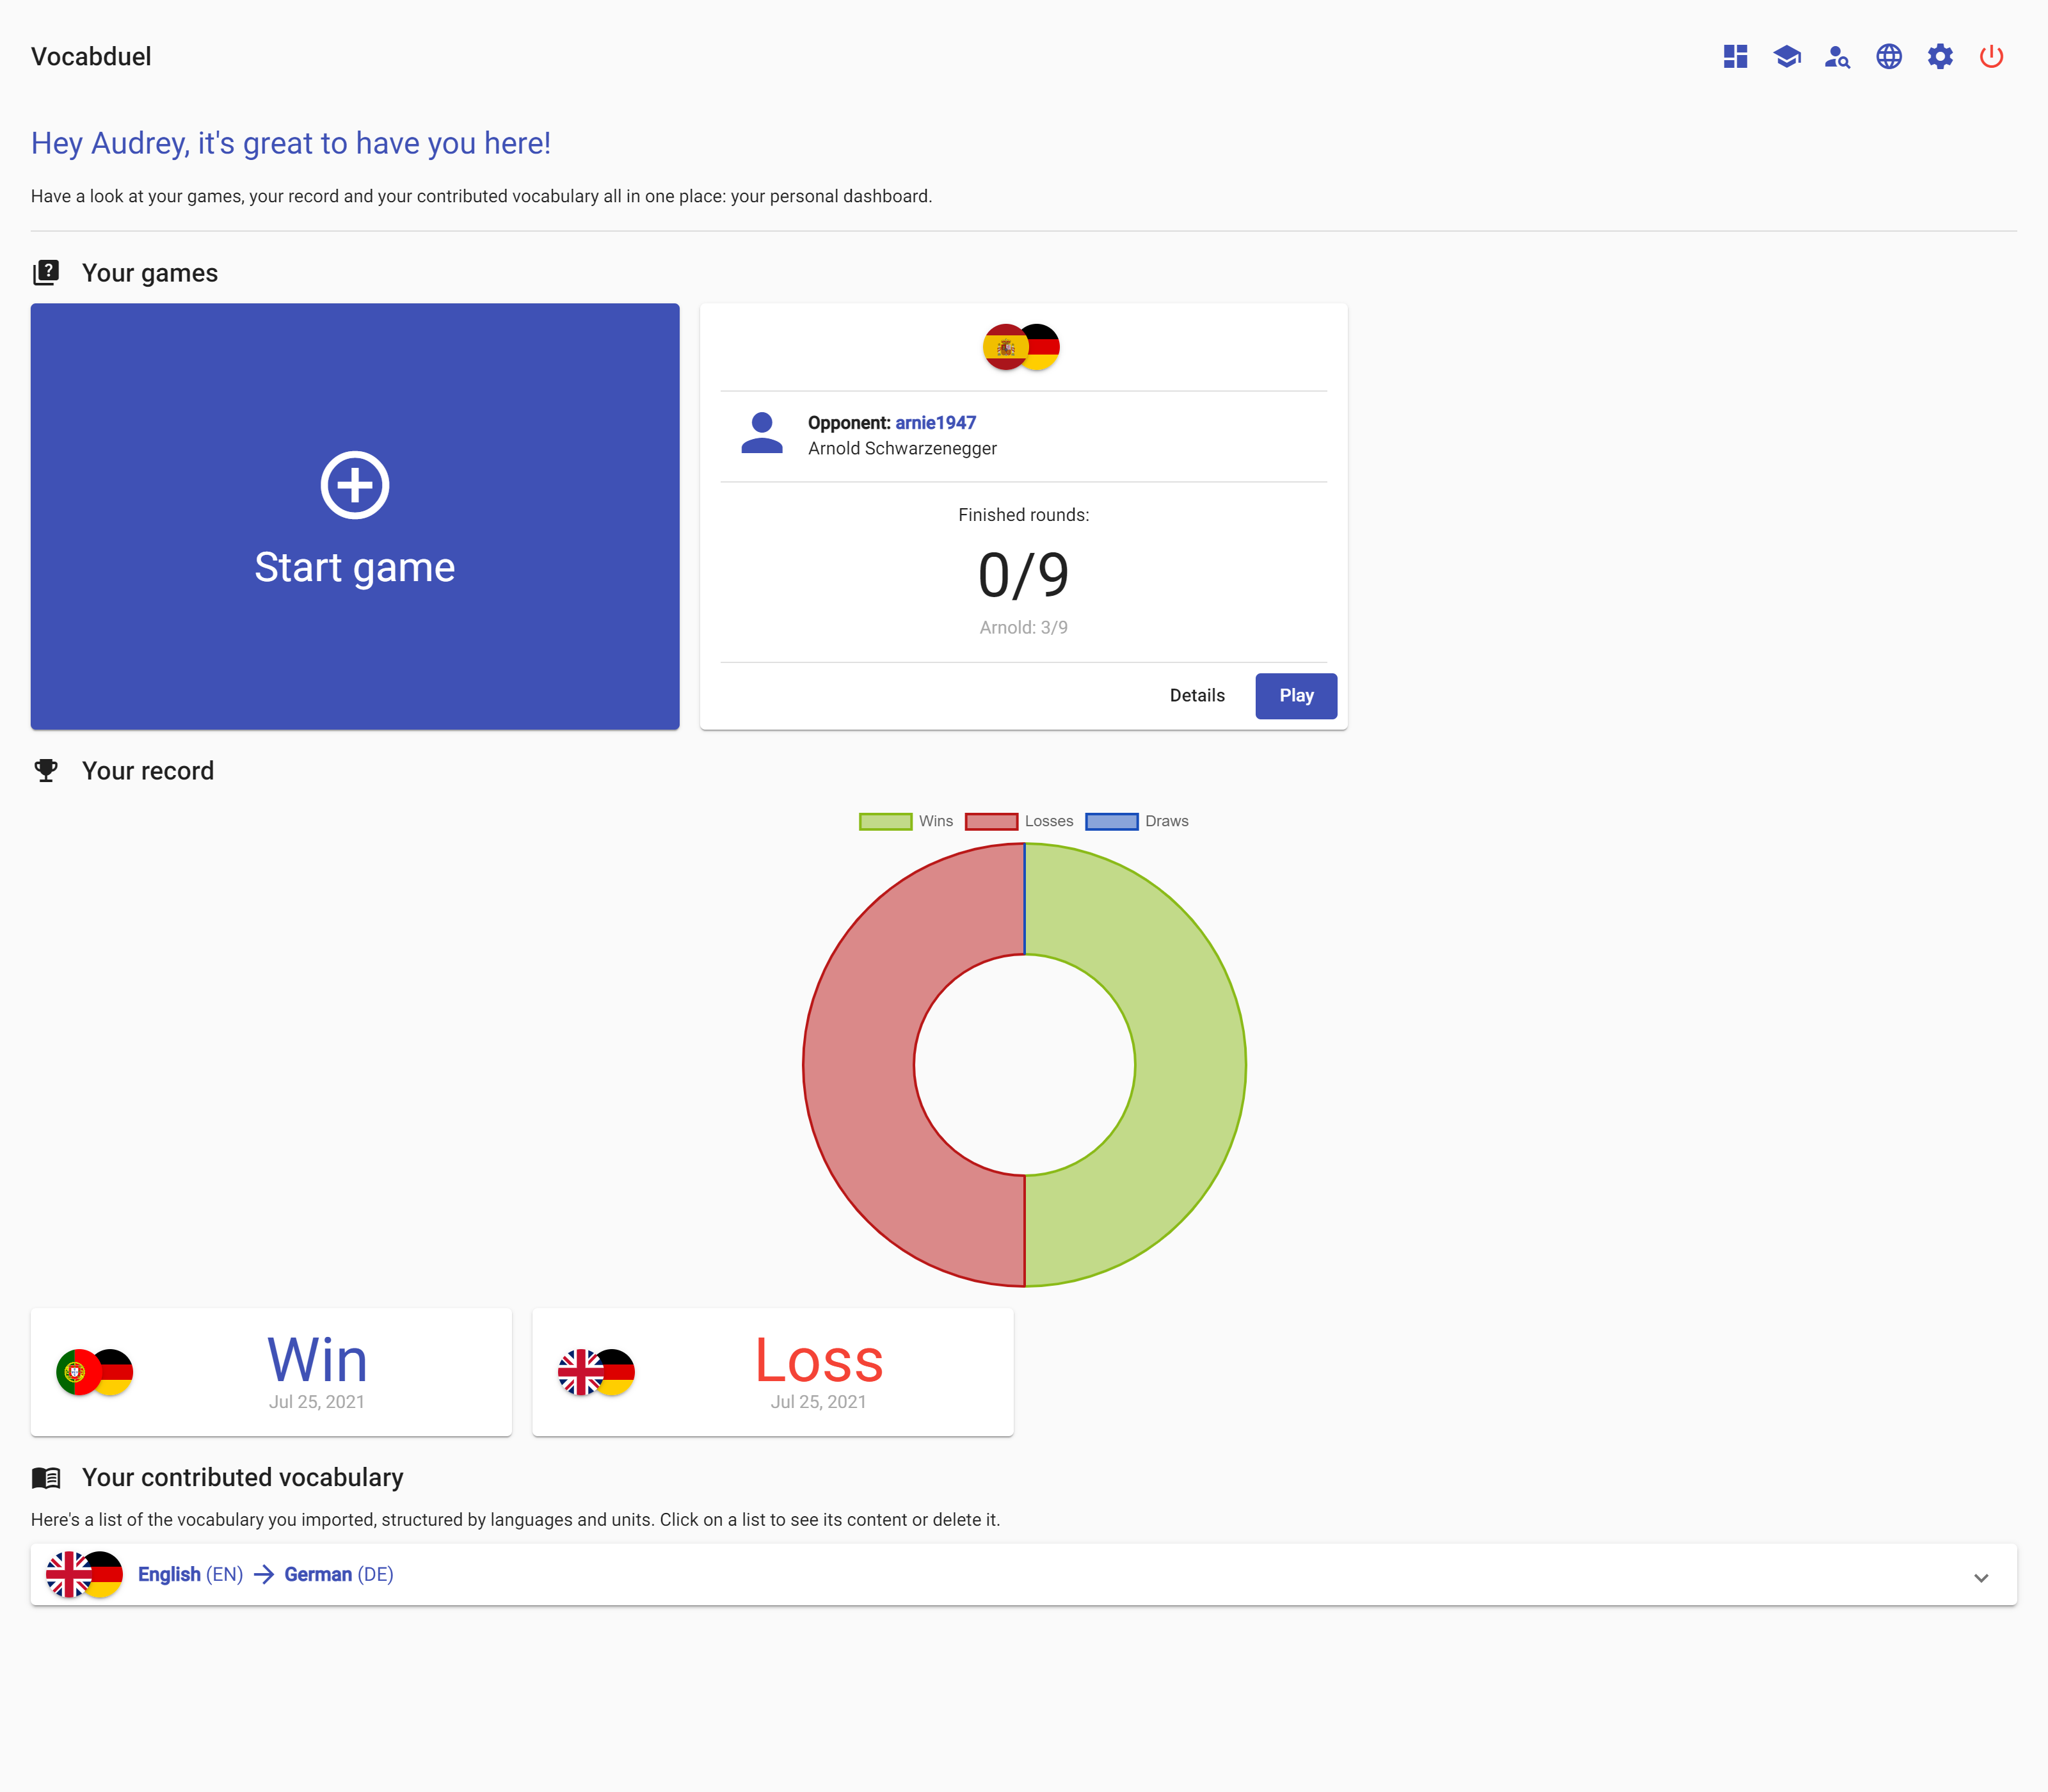
\includegraphics[width=0.8\textwidth]{localhost_8080_appdashboard (1)}
    \caption[]{Dashboard}
    \label{fig:fedashboard}
\end{figure}

Sobald eingeloggt, besteht Zugriff auf das persönliche Dashboard, das aktuelle Spiele, Spielergebnisse sowie eine Übersicht
über vom angemeldeten Nutzer importierte Vokabellisten beinhaltet.

\begin{figure}[H]
    \centering
    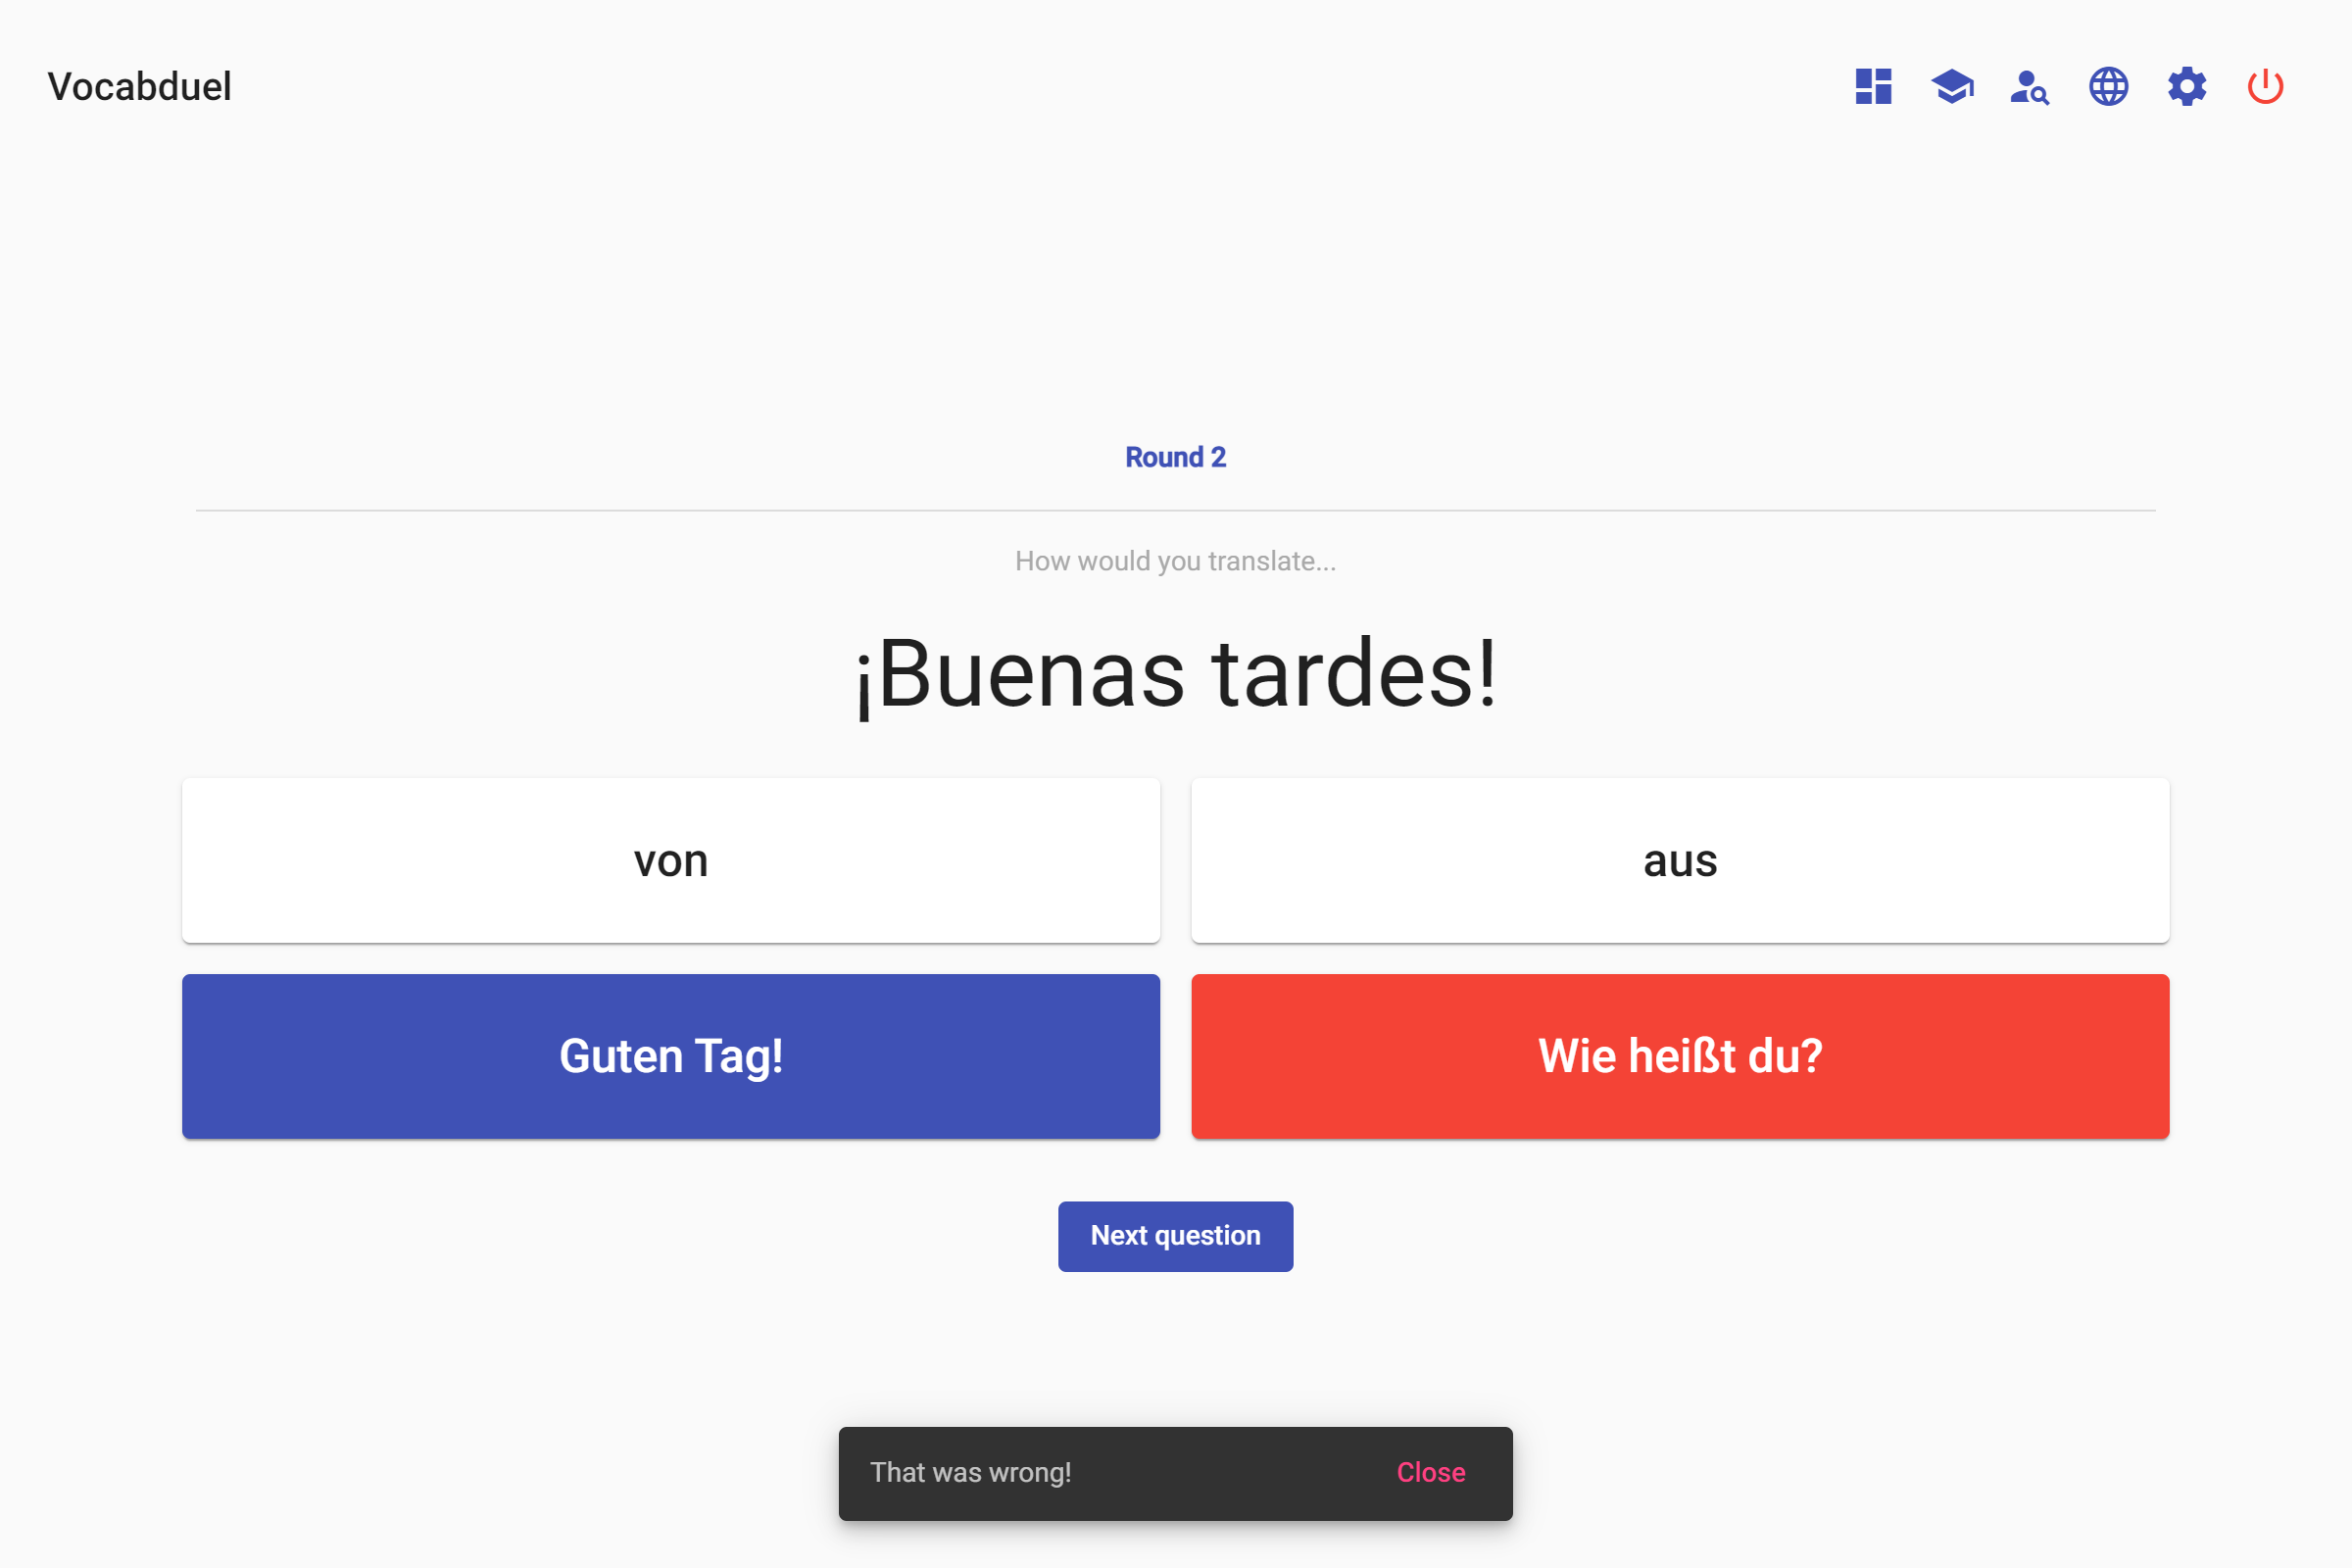
\includegraphics[width=0.8\textwidth]{localhost_8080_app_login (2)}
    \caption[]{Beantworten einer Frage}
    \label{fig:fegame}
\end{figure}

Vom Dashboard aus kann entweder ein existierendes Spiel geöffnet oder ein neues Spiel gestartet werden.
Nach dem Einreichen einer Antwort erfolgt direktes Feedback und die nächste Runde (sofern vorhanden) kann
gespielt werden.

\begin{figure}[H]
    \centering
    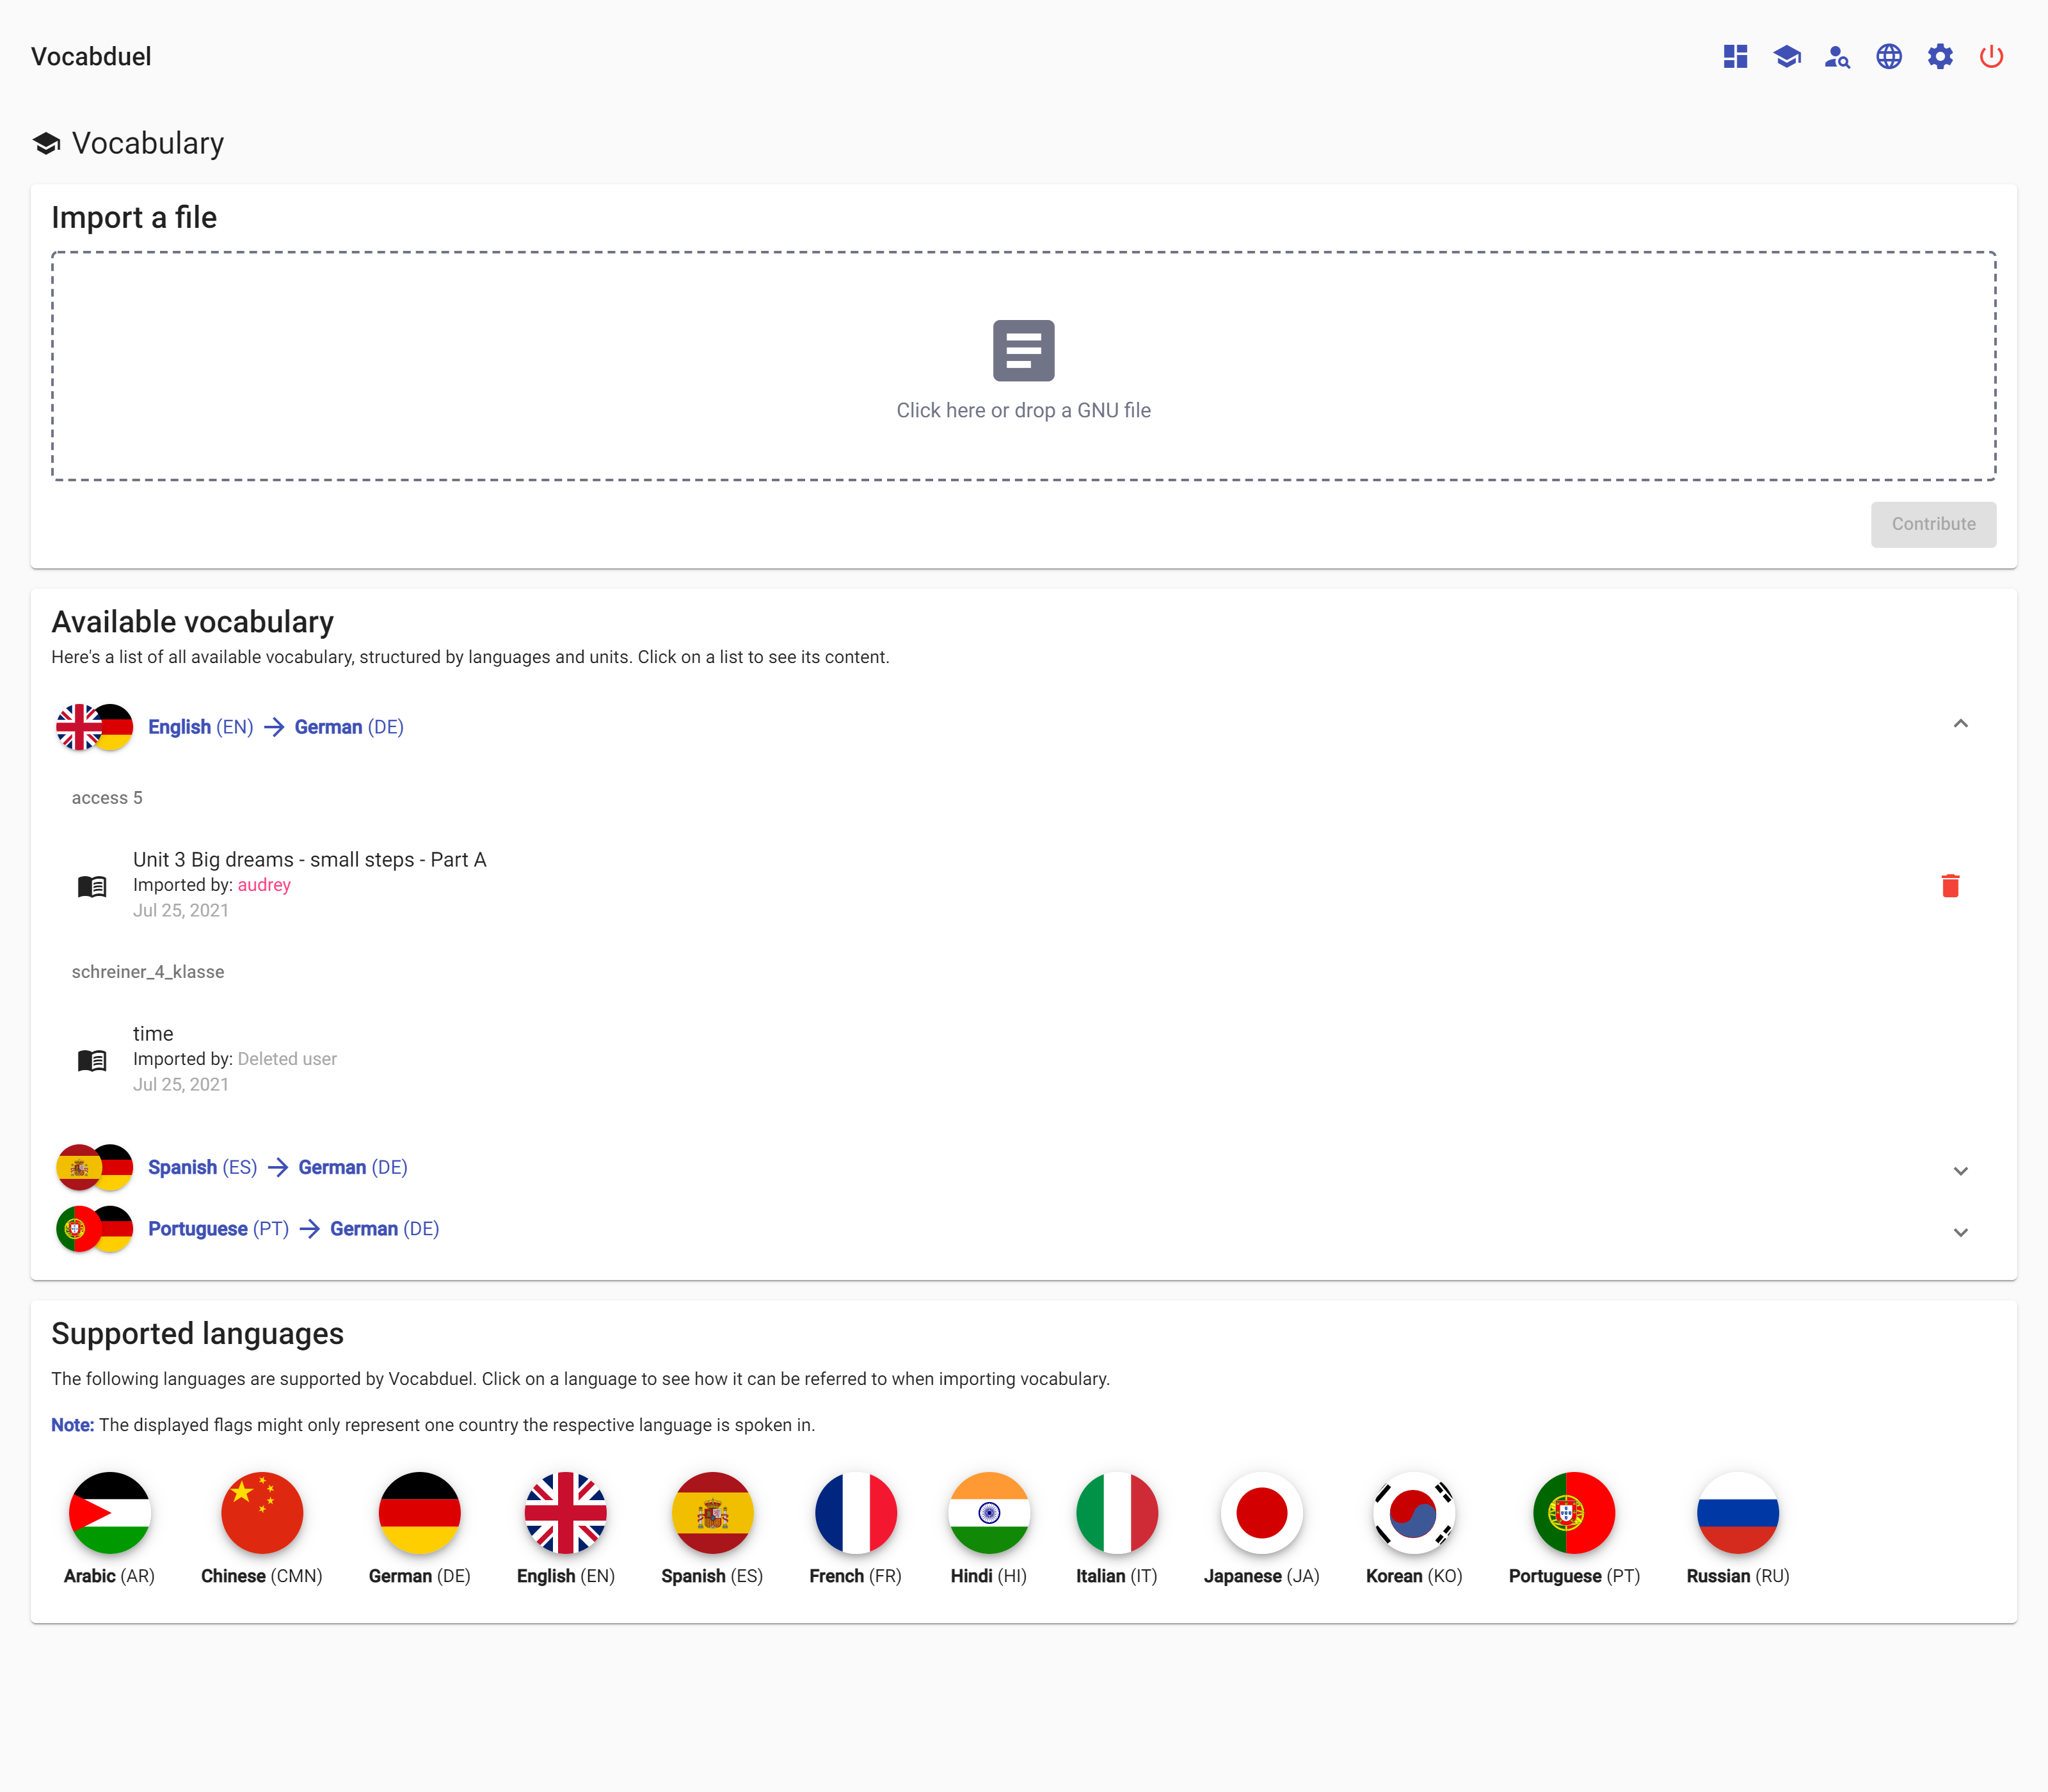
\includegraphics[width=0.8\textwidth]{localhost_8080_app_vocab}
    \caption[]{Vokabelmanagement}
    \label{fig:fevocab}
\end{figure}

Die Vokabelmanagement-Seite zeigt alle importierten Vokabellisten, gruppiert nach Sprachen und Units sowie alle vom System
unterstützen Sprachen für Vokabellisten.
Grundsätzlich ist sie ohne vorherige Authentifizierung zugänglich, in diesem Fall könnten allerdings keine neuen Vokabellisten importiert werden (vgl.\ Abbildung~\ref{fig:fevocab}).

\begin{figure}[H]
    \centering
    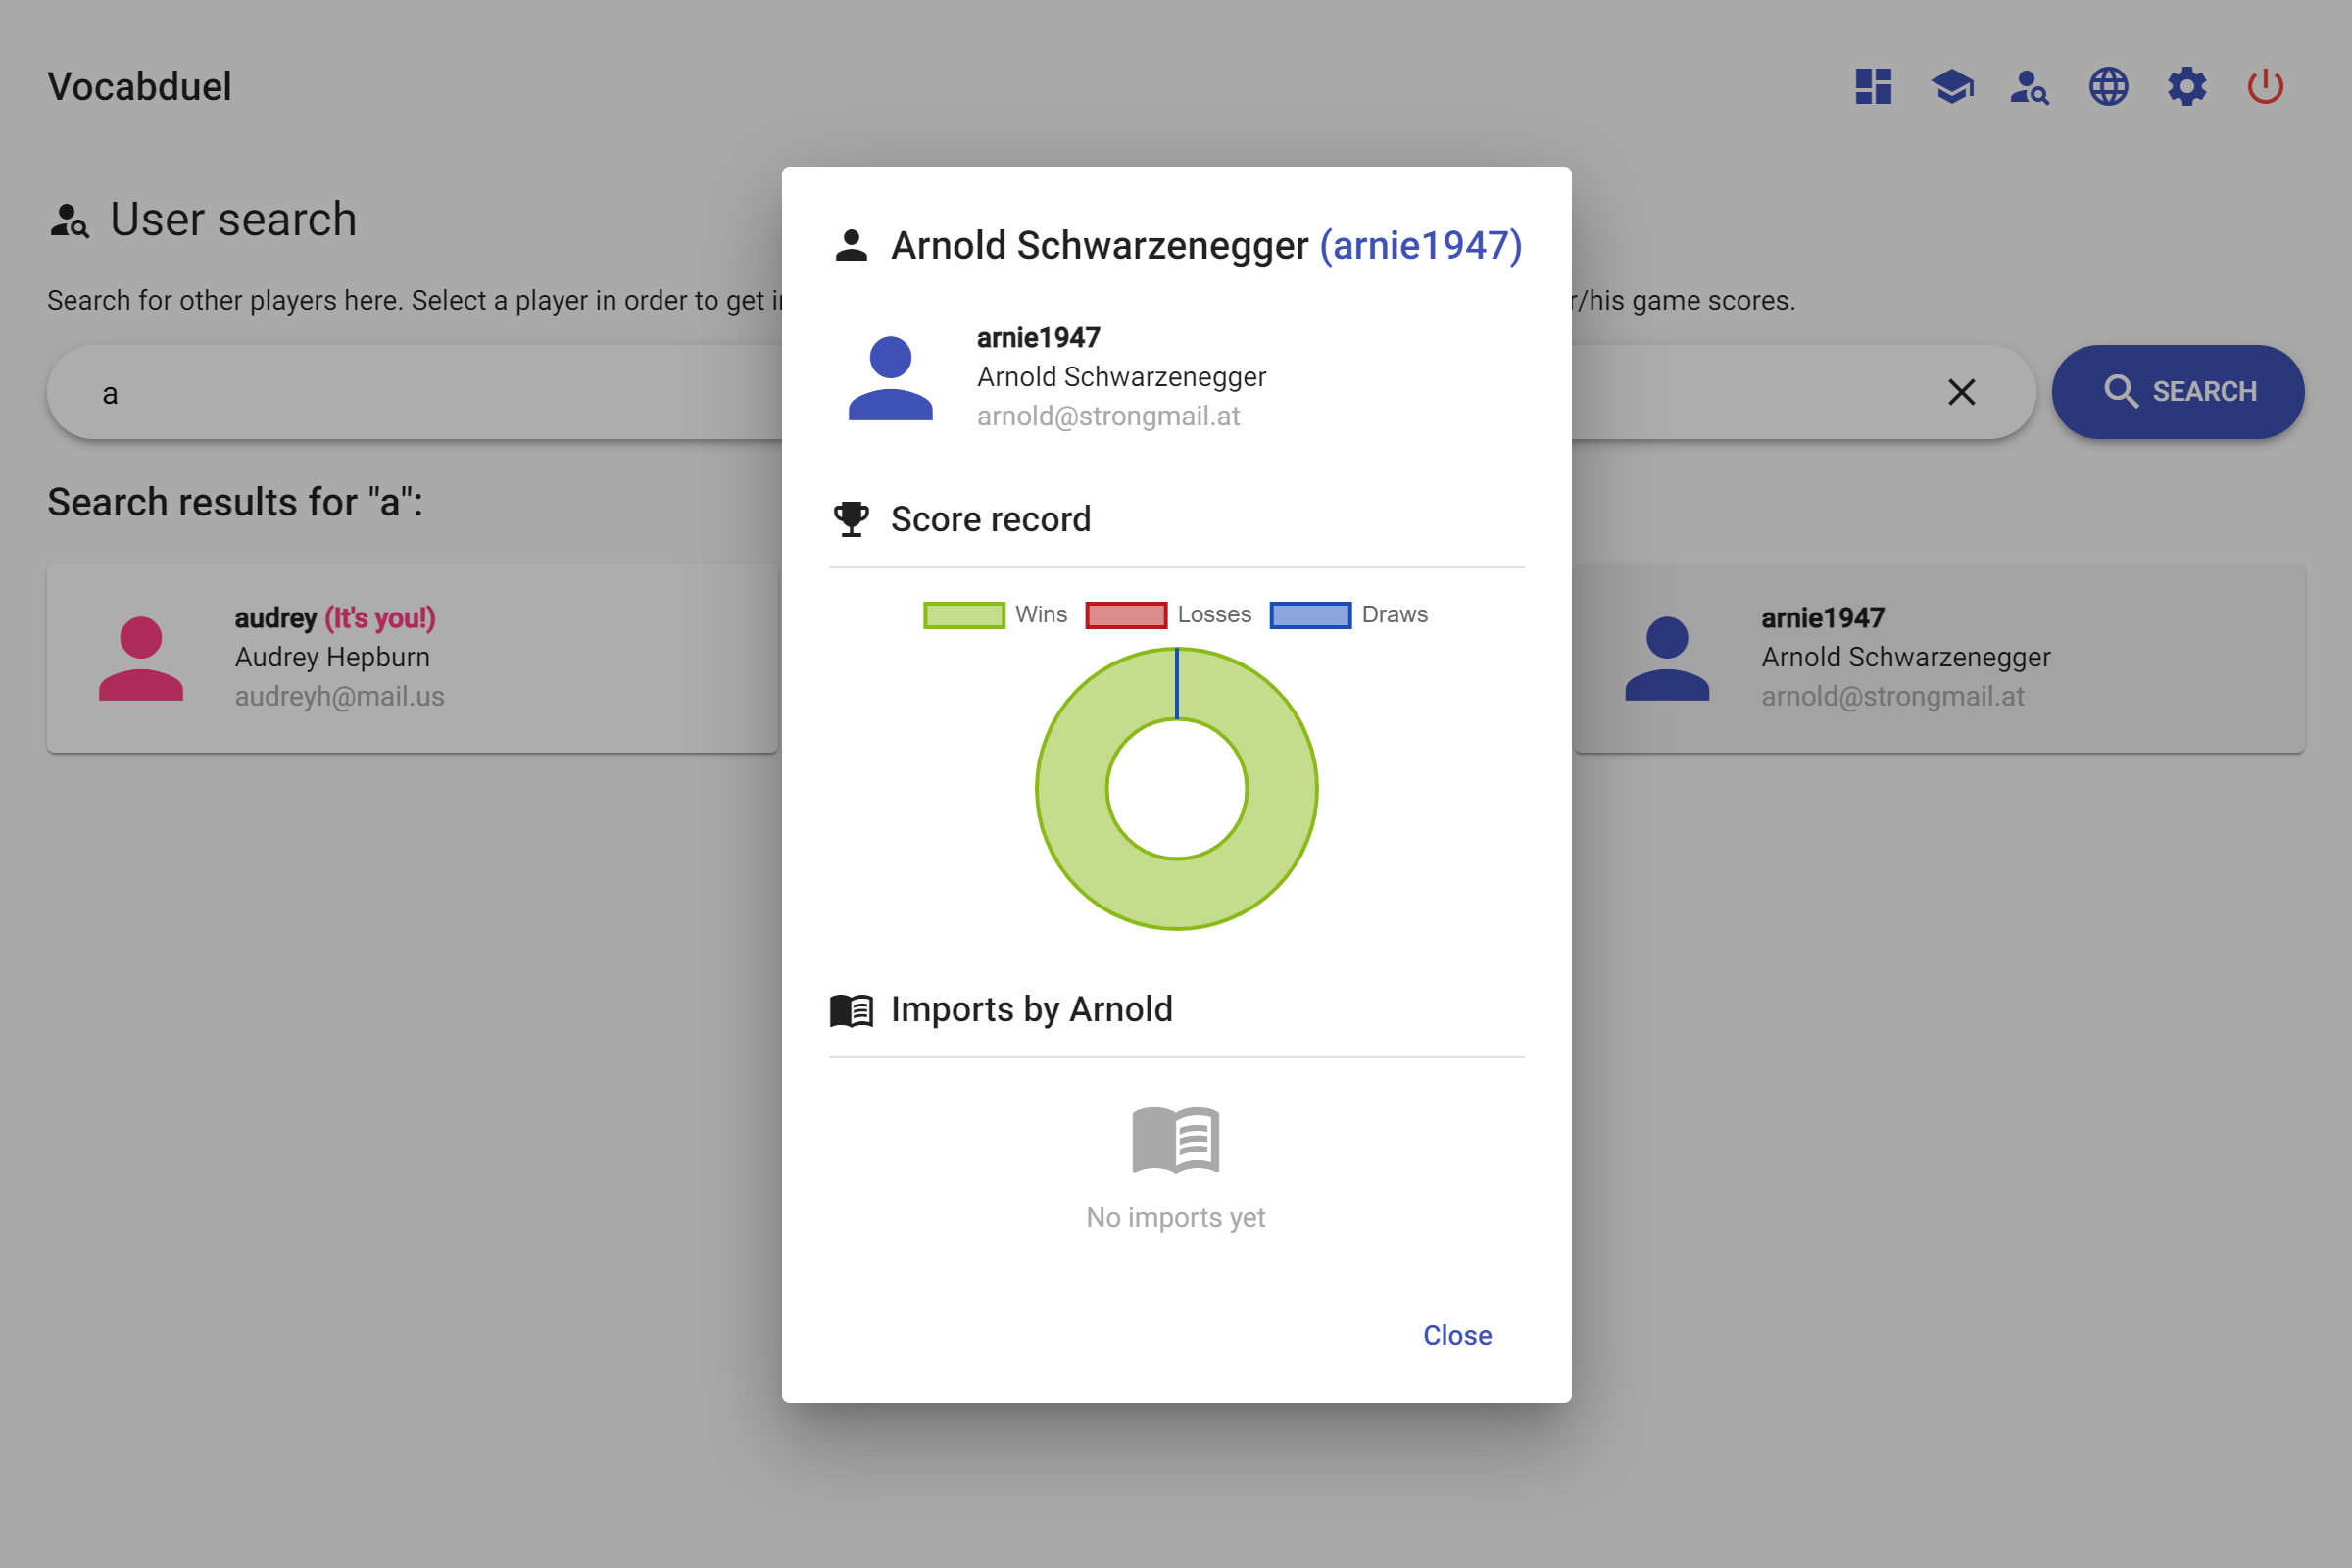
\includegraphics[width=0.8\textwidth]{localhost_8080_app_search}
    \caption[]{Details zu einer gesuchten Person}
    \label{fig:fesearch}
\end{figure}

Ähnlich ist die Suche nach Nutzern frei zugänglich.
Die Spielergebnisse einer Person sehen zu dürfen, setzt allerdings eine Authentifizierung voraus, während von der ausgewählten Person importierte Listen öffentlich einsehbar sind.
Um Details zu einem Datensatz wie einem Spiel, einer Vokabelliste oder, wie hier, einer Person einzusehen, finden in der Anwendung Dialoge Verwendung.

\begin{figure}[H]
    \centering
    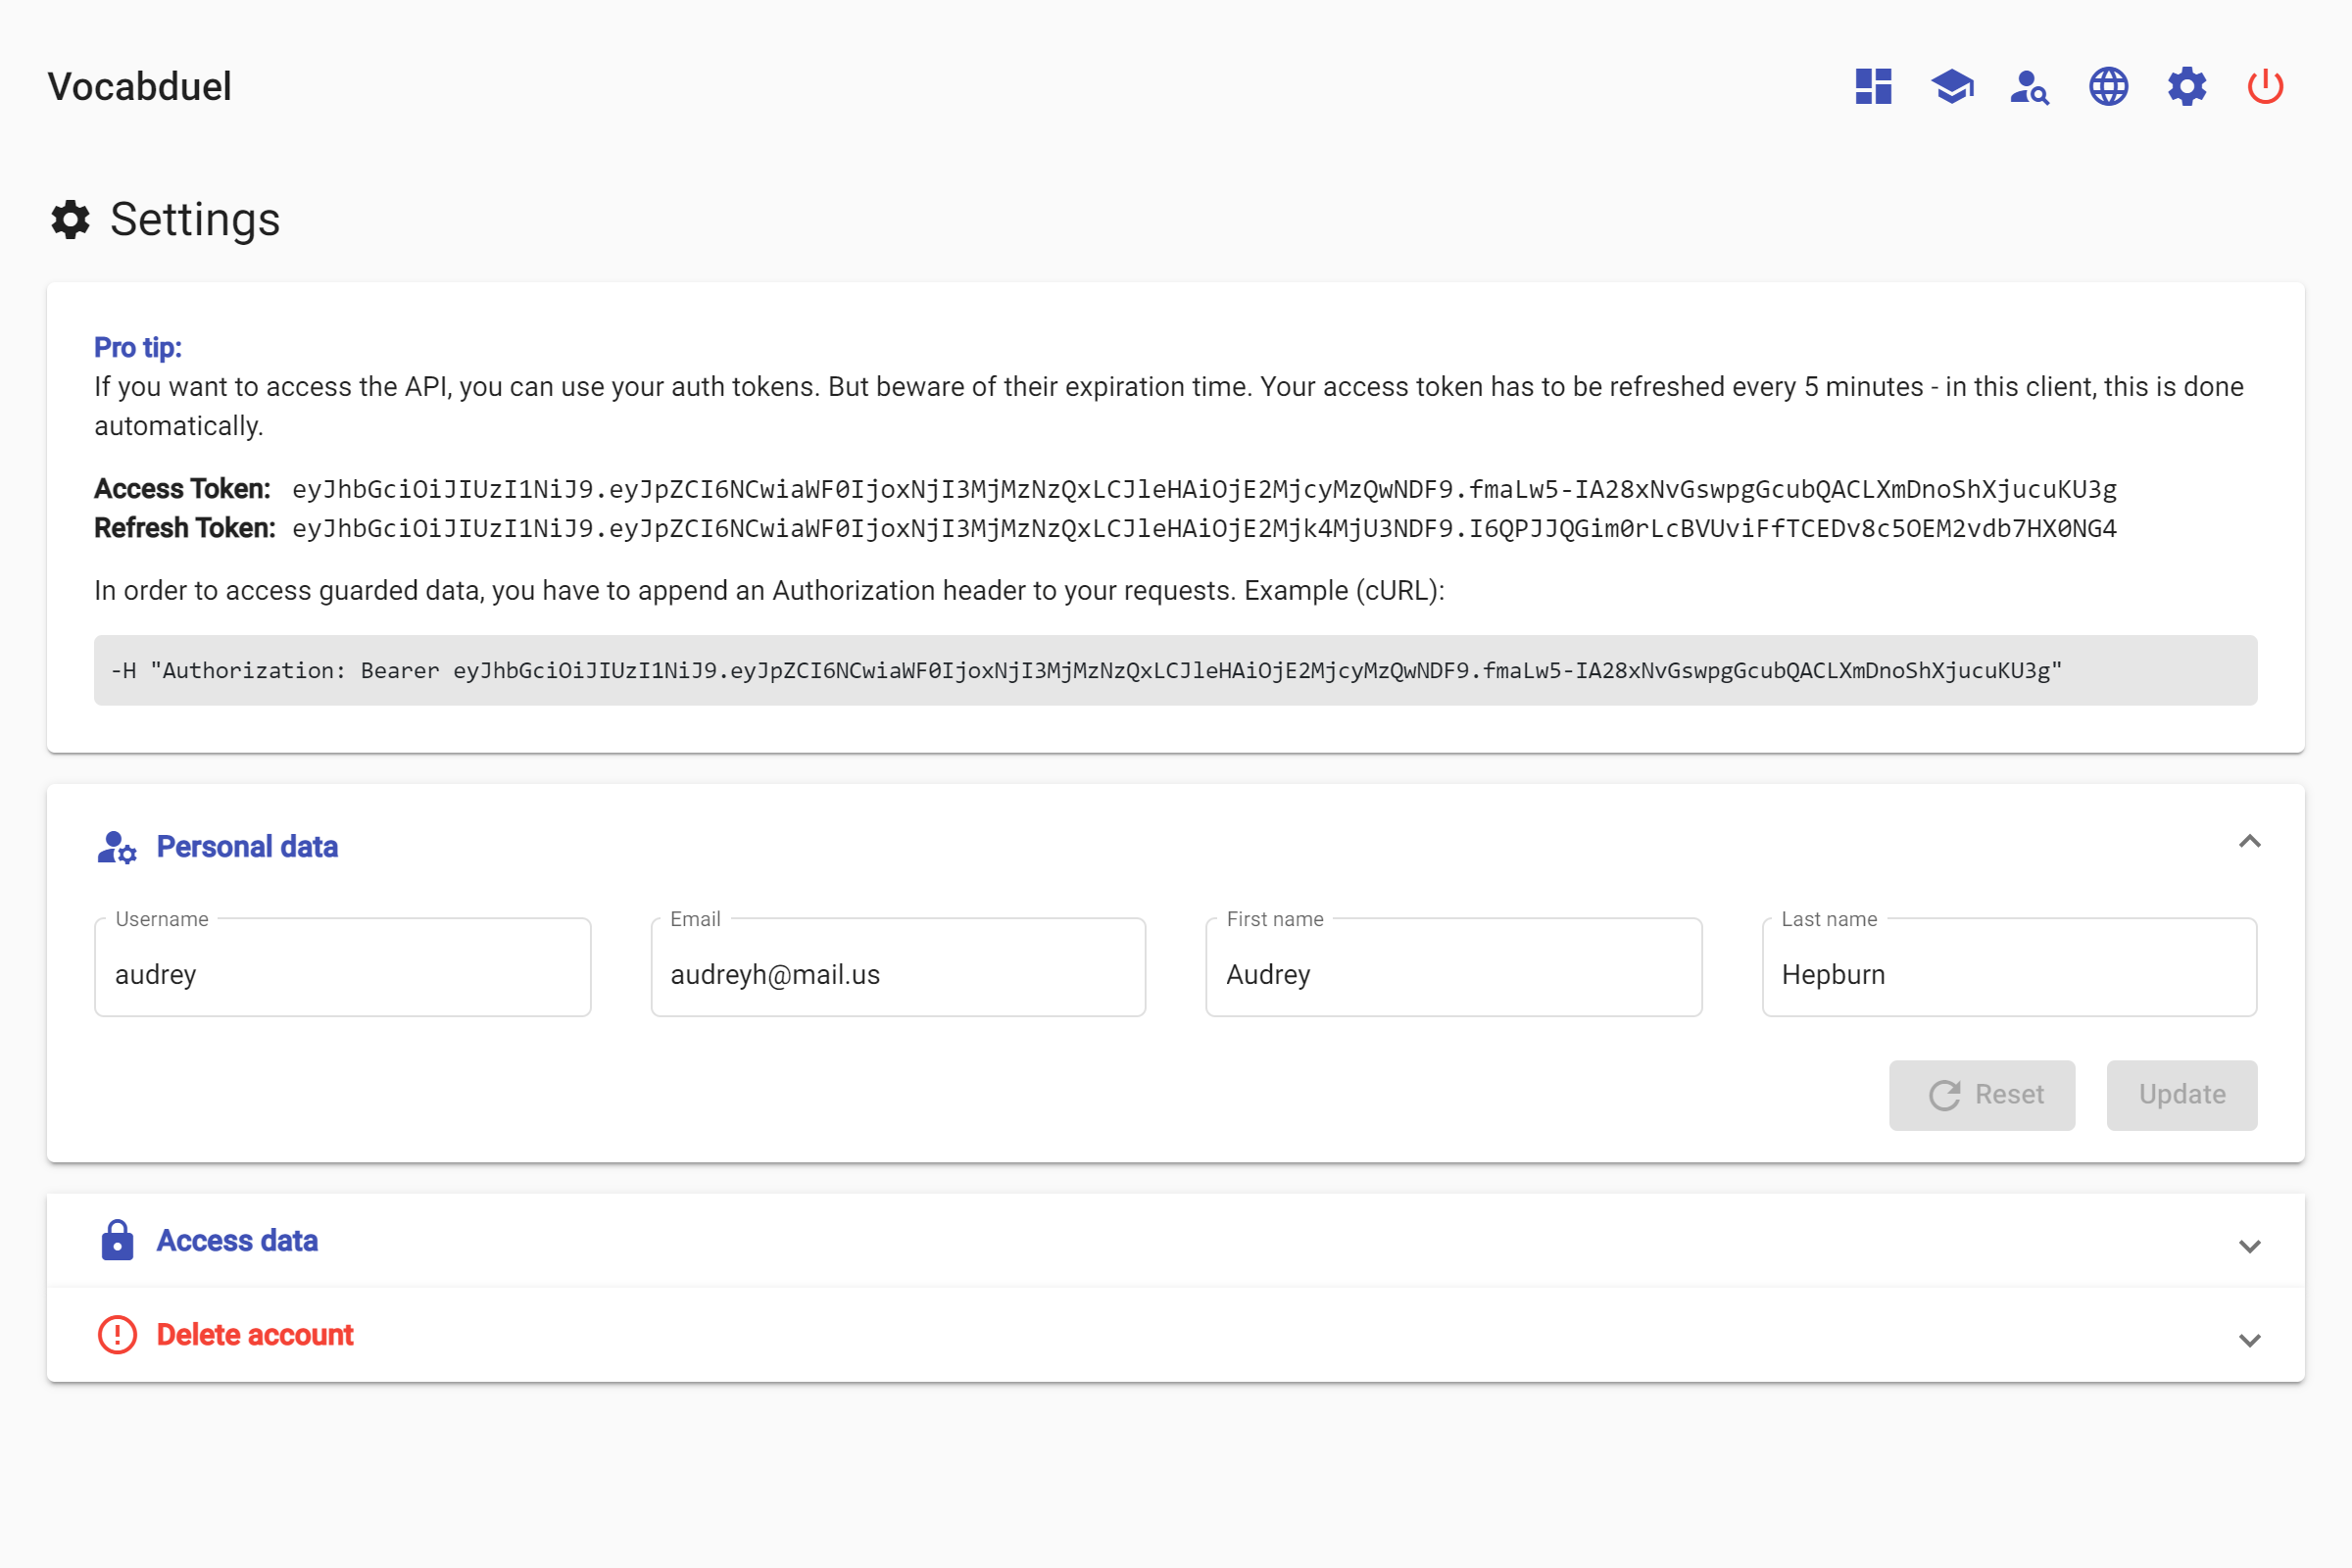
\includegraphics[width=0.8\textwidth]{localhost_8080_app_login (1)}
    \caption[]{Nutzereinstellungen}
    \label{fig:fesettings}
\end{figure}

Sofern authentifiziert, besteht zudem die Möglichkeit, persönliche Daten über die Nutzereinstellungen zu konfigurieren.

\subsubsection{Struktur aus Entwicklungssicht}

Aus Entwicklungssicht besteht die Anwendung aus:

\begin{itemize}
    \item \textbf{Components:} Anzuzeigende Komponenten, die jeweils aus einer \textit{HTML}-, einer \textit{SCSS-}
    und einer \textit{TypeScript}-Datei bestehen. Diese sind beliebig wiederverwertbar und lassen sich ineinander verschachteln.
    Zusammengefasst sind somit alle dargestellten Bestandteile der Anwendung Components, die Teil der \texttt{AppComponent} sind.
    \item \textbf{Directives:} Klassen, die dargestellte Elemente um Logik erweitern. In der konkreten Anwendung gibt es lediglich
    eine Directive, die zu langen Text automatisch abbricht und durch "..." ersetzt.
    \item \textbf{Guards:} Interfaces, die prüfen, ob eine bestimmte Route aktiviert werden kann und sollte die hierfür
    aufgestellte Bedingung nicht erfüllt sein, auf eine andere Seite weiterleiten. Ein Beispiel wäre die Login-Seite, die nur
    dann aufgerufen werden kann, wenn keine Person in der aktuellen Session eingeloggt ist. Auch lassen sich für eine Route mehrere
    Guards definieren.
    \item \textbf{Helpers:} Nicht direkt zuordenbare Hilfsklassen. In der konkreten Anwendung gibt es nur eine derartige
    Klasse, die die Authentifizierungslogik für jegliche Requests übernimmt.
    \item \textbf{Model:} Klassen, die die Struktur der verarbeiteten bzw. dargestellen Informationen definieren.
    \item \textbf{Pipes:} Klassen, die dazu dienen, anzuzeigende Werte zu transformieren.
    \item \textbf{Services:} Per DI injizierbare und somit als Singleton nutzbare Klassen, die grundlegende, gemeinsam genutzte
    Logik bereitstellen. In dieser Anwendung ist für jedes REST-Modul eine derartige Serviceklasse definiert, um alle HTTP-Requests
    zentral zu definieren und von den angezeigten Komponenten zu trennen. Weitere Logik wie eine zentrale Verwaltung zum Speichern
    von Daten oder der Sprachenverwaltung (Internationalisierung) ist auch über Serviceklassen realisiert.
\end{itemize}

Das \textit{Vocabduel}-Frontend wurde zunächst als gesondertes Projekt behandelt, im Laufe der Zeit allerdings in das Mono-Repository integriert.
Die Gründe hierfür werden in Kapitel~\ref{sec:ablaufumgebung} näher erläutert.

\subsubsection{Kommunikation mit REST-Schnittstellen}

Die folgende Liste gibt Auskunft darüber, welche REST-Adapter zu welchem Zeitpunkt von der Webanwendung angesprochen werden bzw.\ durch Nutzerinteraktionen ansprechbar sind:

\begin{outline}
    \1 \textbf{\texttt{AuthServiceRestAdapter}}
    \2 \texttt{/register} : Registrierungsseite
    \2 \texttt{/login} : Loginseite
    \2 \texttt{/current-user} : \textit{(Anzahl an Requests durch clientseitiges Caching eingeschränkt)}
    \3 Jede Seite, die Authentifizierung erfordert
    \3 Guards zum Prüfen, ob authentifiziert
    \2 \texttt{/refresh-token} : Im Hintergrund bei Error \texttt{401} (\texttt{AuthInterceptor})
    \2 \texttt{/update-password} : Nutzereinstellungen

    \1 \textbf{\texttt{UserServiceRestAdapter}}
    \2 \texttt{/find} :
    \3 Seite zur Suche nach Personen
    \3 Dialog für die Festlegung eines Gegners beim Starten eines Spiels
    \2 \texttt{/get} : Dialog für die Festlegung eines Gegners beim Starten eines Spiels
    \2 \texttt{/update-account} : Nutzereinstellungen

    \1 \textbf{\texttt{VocabularyServiceRestAdapter}}
    \2 \texttt{/list/\{id\}} : Vokabelliste-Dialog, wenn von Spieldetails aus geöffnet
    \2 \texttt{/lists-of-author/\{id\}} :
    \3 Dashboard (eigene Listen)
    \3 User-Details-Dialog
    \2 \texttt{/language-sets} :
    \3 Vokabelmanagement-Seite
    \3 Dialog zur Auswahl von Vokabellisten beim Starten eines Spiels
    \2 \texttt{/language-references/\{lang\}} : Vokabelmanagement-Seite
    \2 \texttt{/supported-languages} : Vokabelmanagement-Seite
    \2 \texttt{/import-gnu} : Vokabelmanagement-Seite
    \2 \texttt{/delete-list/\{listId\}} :
    \3 Vokabelmanagement-Seite
    \3 Dashboard (eigene Listen)

    \1 \textbf{\texttt{GameServiceRestAdapter}}
    \2 \texttt{/finish-game} : Seite mit laufendem Spiel
    \2 \texttt{/finished-games} : Dashboard
    \2 \texttt{/record} : Dashboard
    \2 \texttt{/record/{userId}} : User-Details-Dialog

    \1 \textbf{\texttt{GameServiceRestAdapter}}
    \2 \texttt{/start} : Seite zum Starten eines Spiels
    \2 \texttt{/open-games} : Dashboard
    \2 \texttt{/current-round/\{gameId\}} : Seite mit laufendem Spiel
    \2 \texttt{/answer/\{gameId\}/\{roundNr\}} : Seite mit laufendem Spiel
    \2 \texttt{/delete-account-and-game-widows} : Nutzereinstellungen

\end{outline}

\textbf{Anmerkung:} Das Löschen von Nutzerdaten über \texttt{GameServiceRestAdapter} zu steuern, ermöglicht es, direkt
alle zugehörigen offenen Spiele der gelöschten Person zu entfernen.

\subsubsection{Fehlerbehandlung}

In der Anwendung existiert ein zentraler Service, der alle unbehandelten Fehler abfängt (\texttt{ErrorService}), für die abhängig vom Statuscode (sofern vorhanden) einen
bestimmten, generischen Dialog anzeigt.

\begin{figure}[H]
    \centering
    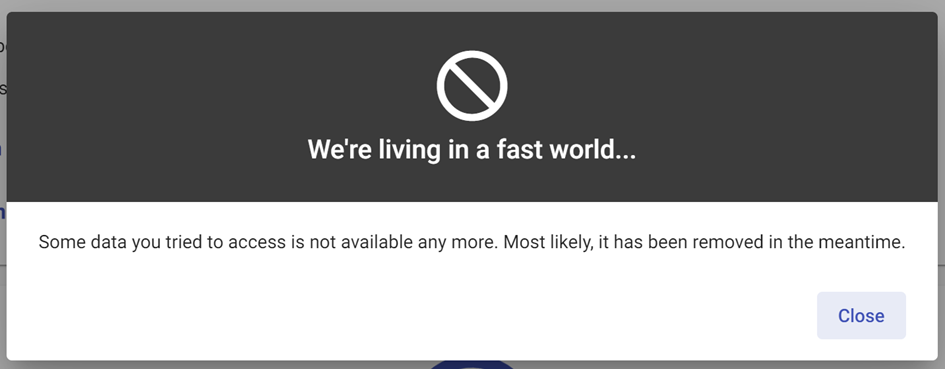
\includegraphics[width=0.8\textwidth]{404-dialog}
    \caption[]{Generische Behandlung eines \texttt{Not Found} Errors (404)}
    \label{fig:404}
\end{figure}

\begin{figure}[H]
    \centering
    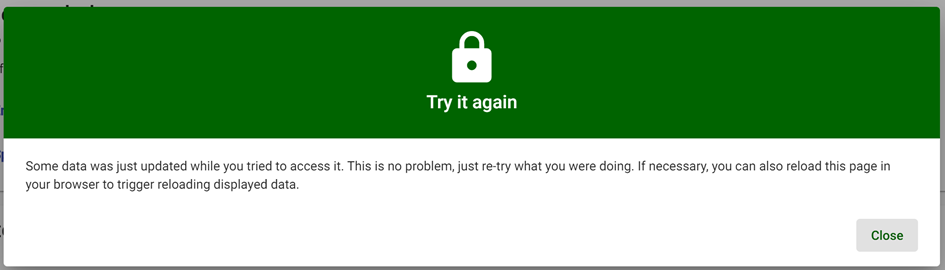
\includegraphics[width=0.8\textwidth]{412-dialog}
    \caption[]{Generische Behandlung eines \texttt{Precondition Failed} Errors (412)}
    \label{fig:412}
\end{figure}

\begin{figure}[H]
    \centering
    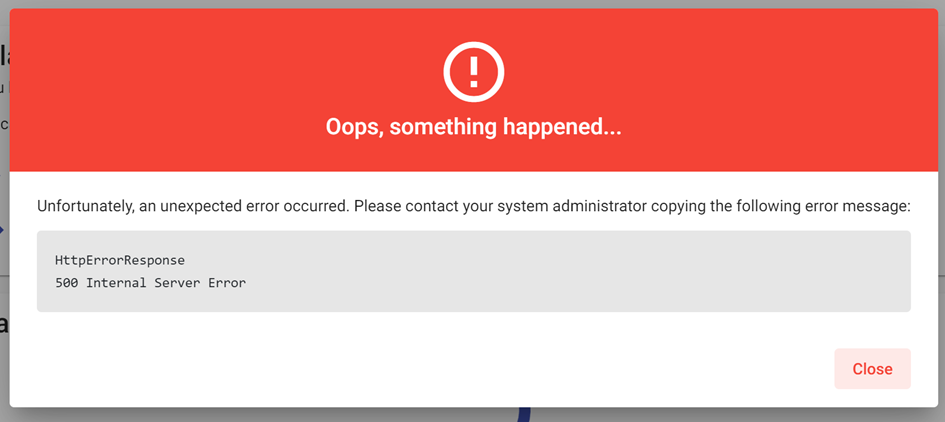
\includegraphics[width=0.8\textwidth]{500-dialog}
    \caption[]{Generische Behandlung eines unerwarteten Fehlers, in diesem Beispiel \texttt{Internal Server Error (500)} (anzunehmender Regelfall)}
    \label{fig:500}
\end{figure}

Darüber hinaus werden \texttt{Bad Request} Errors (400) in der Regel wie folgt behandelt:

\begin{figure}[H]
    \centering
    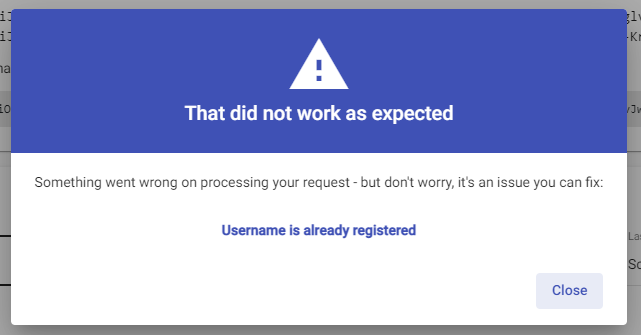
\includegraphics[width=0.8\textwidth]{400-dialog}
    \caption[]{Typische Behandlung eines \texttt{Bad Request} Errors (400)}
    \label{fig:400}
\end{figure}

\subsubsection{Weitere Features}

Die Anwendung ist so implementiert, dass sie sowohl auf kleinen als auch auf großen Bildschirmen verwendet werden kann (Responsive Design)
und orientiert sich in ihrer allgemeinen Erscheinung stark an Guidelines und Best Practices zu Material Design.

Des Weiteren ist die Applikation aktuell nur auf Englisch verfügbar, allerdings durch das Auslagern von Strings sowie einen vollständig implementierten
Service zum Verwalten von Sprachdateien (\texttt{I18nService}) leicht in andere Sprachen zu übersetzen.

\subsection{Postman Collection}

Zum Testen der API ist auch eine \textit{Postman}-Collection mit vordefinierten Requests im Rootverzeichnis des Repositorys hinterlegt.
Für Nutzer mit den IDs 2, 4 und 6, die in den ersten Requests angelegt werden, sind Tokens mit einer Gültigkeit von
5 Jahren konfiguriert, um die eigentlich implementierte regelmäßige Neuauthentifizierung bei der Nutzung der Collection zu umgehen.
